\section{Feature-Auswahl, Hyperparametersuche und Modellauswahl} \label{sec:Ergeb FeatSel,Hyp,ModSel}
Um eine optimale Feature-Menge zu finden, wird aus einer Reihe von Versuchen mit Wrapper-Methoden eine Feature-Rangfolge abgeleitet. Um die Feature-Menge unabhängig vom Modell zu beurteilen, wird die Accuracy von mehreren Modellen validiert und anschließend gemittelt. In diesem Kapitel werden die Feature-Rangfolgen der Filter-Methoden betrachtet. Damit wird die konstruierte Rangfolge aus dem Wrapper-Score verglichen. Es wird untersucht, ob sich das Entfernen von Features, die auf dem gleichen Basis-Feature aufbauen, positive auswirkt. Ebenfalls wird untersucht, ob alle Feature-Kategorien benötigt werden. Abschließend vergleicht das Kapitel die betrachteten Modelle und führt den finalen Test des ausgewählten Modells durch.\par

Das Ziel der Untersuchung besteht darin, das bestmögliche Modell für das Modul zu entwickeln. Dabei wird nach einer Feature-Menge und einem Modell gesucht, die besser performen als andere Feature-Mengen oder Modelle. Dabei ist es wichtig, auch die Verarbeitungszeit zu berücksichtigen. Für das Modul ist eine kleine Feature-Menge vorteilhafter, um die Echtzeitfunktionalität zu gewährleisten. \par


\subsection{Vergleich der Filter-Methoden mit der entworfenen Rangfolge}
Die Plots in Abbildung \ref{fig:plotMethVergl} zeigen den Verlauf der Accuracy in Bezug auf die Feature-Menge gemäß der jeweiligen Rangfolge. Dabei sind die Varianzanalyse, die gegenseitige Information und der Wrapper-Score dargestellt. Zur besseren Vergleichbarkeit sind die Sättigungskurve eingezeichnet. Die Tabelle \ref{tab:FiltVsWrap} zeigt einen tabellarischen Vergleich der Ergebnisse.

\begin{figure}[htbp]
     \centering
     \begin{subfigure}[b]{0.9\textwidth}
         \centering
         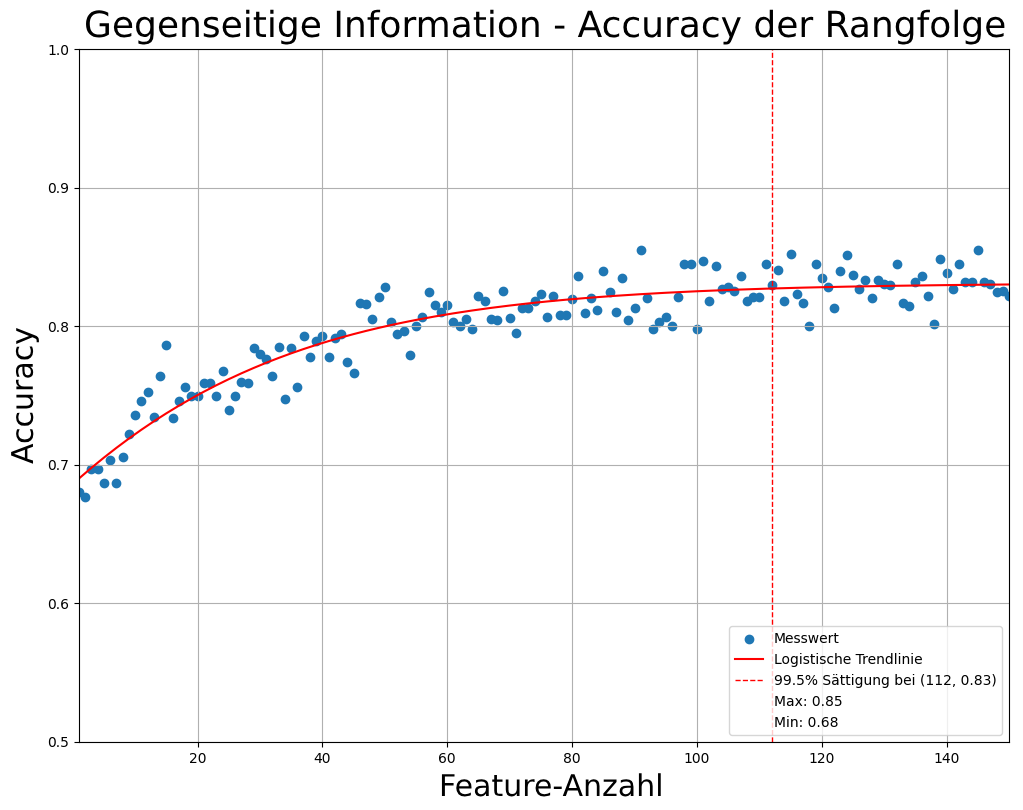
\includegraphics[width=\textwidth, height=11cm]{img/Plots/Feature Auswahl/Filter-Methoden Mutual Info.png}
         \caption{Varianzanalyse}
     \end{subfigure}
     \hfill
     \begin{subfigure}[b]{0.9\textwidth}
         \centering
         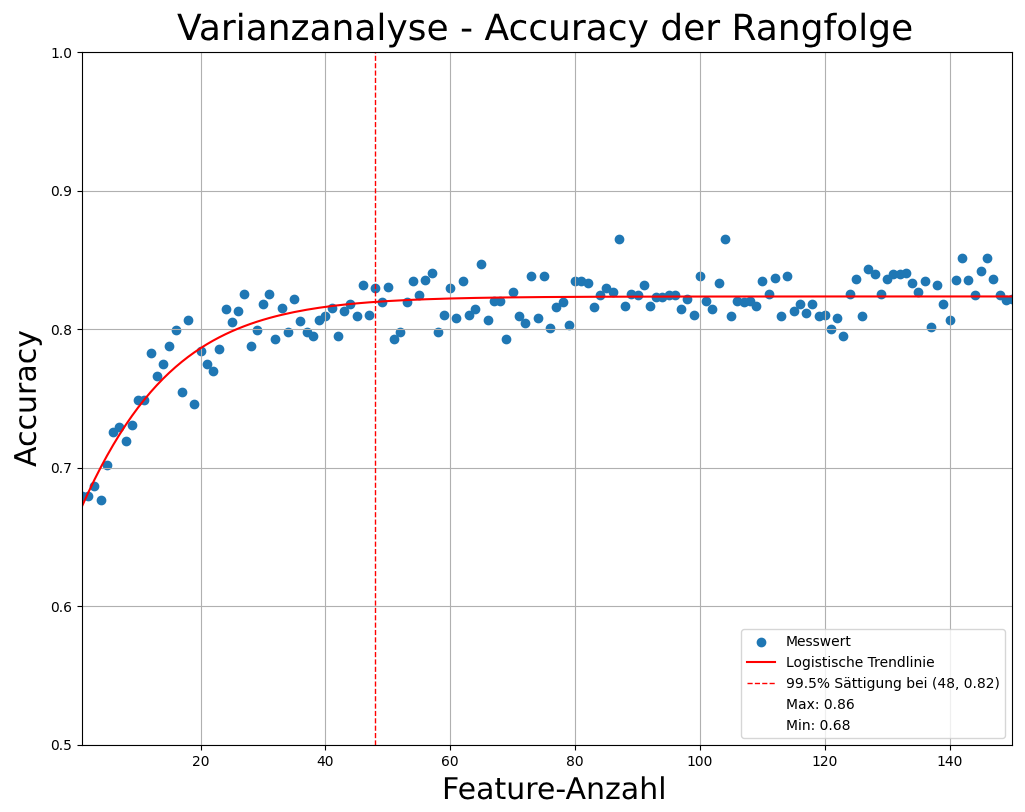
\includegraphics[width=\textwidth, height=11cm]{img/Plots/Feature Auswahl/Filter-Methoden ANOVA.png}
         \caption{Gegenseitige Information}
     \end{subfigure}
     \caption{Verlauf der Accuracy der Filter-Methoden und der entworfenen Rangfolge.}
     \label{fig:plotMethVergl}
\end{figure}

\begin{table}[htbp]
\centering
\caption{Vergleich der Sättigungspunkte der Rangfolgen.}
\label{tab:FiltVsWrap}
\begin{tabular}{
  >{\raggedright\arraybackslash}p{0.4\linewidth}
  S[table-format=2.0]
  S[table-format=3.0]
}
\toprule
{Methode} & {Accuracy [\%]} & {Featureanzahl} \\
\midrule
Varianzanalyse & 82 & 48 \\
gegenseitige Information & 83 & 112 \\
Wrapper-Score & 85 & 36 \\
\bottomrule
\end{tabular}
\end{table}

Es ist zu sehen, dass die Rangfolge nach dem Wrapper-Score zu einem optimalen Verlauf der Accuracy resultiert. Die Sättigung wird mit der kleinsten Feature-Menge erreicht und die Accuracy ist im Vergleich am höchsten. Das legitimiert das angewandte Vorgehen. \par

Wie in \autoref{sec:Meth KonstrFeatures} dargestellt, liegt die Feature-Anzahl bei 3114. Die Plots zeigen, dass nur ein Bruchteil dieser Menge notwendig ist, um die Sättigung zu erreichen. Das deutet auf eine hohe Redundanz in den Features hin.


\subsection{Auswirkungen der Entfernung von Features gleicher Basis} \label{sec:Ergeb FeatKategories}

\begin{figure}[hp]
     \centering
     \begin{subfigure}[b]{0.9\textwidth}
         \centering
         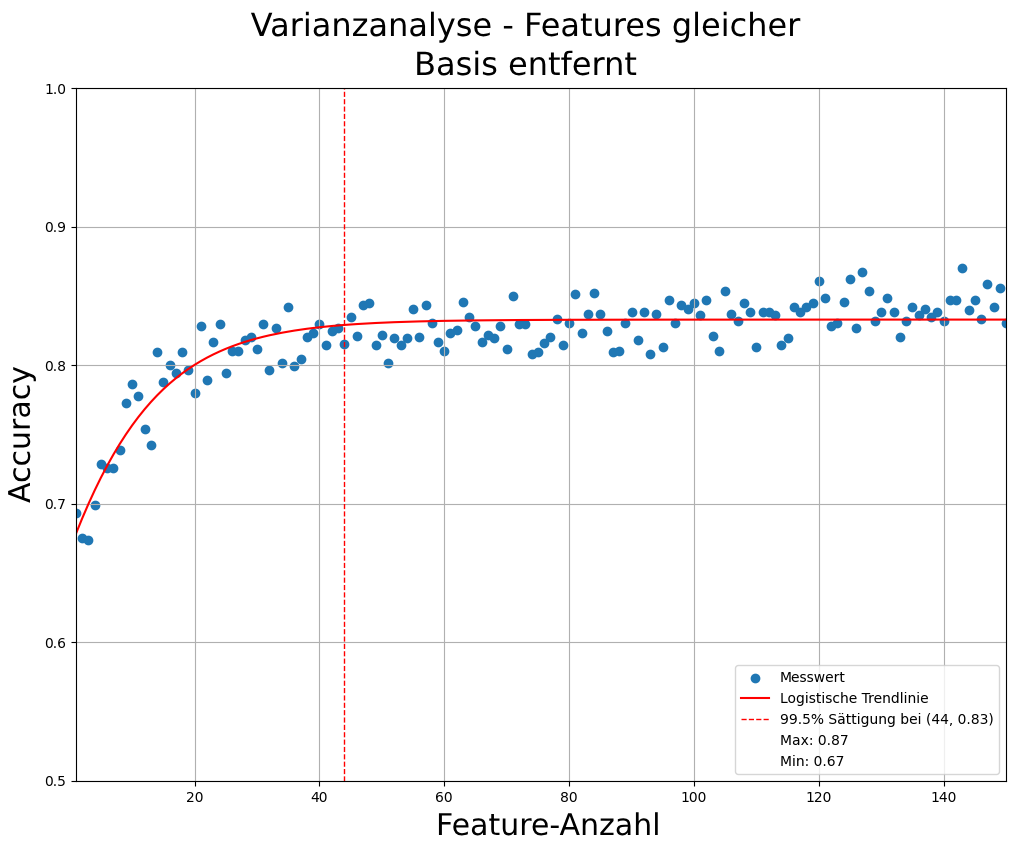
\includegraphics[width=\textwidth, height=11cm]{img/Plots/Feature Auswahl/Filter-Methoden ANOVA mit Entfernen.png}
         \caption{Varianzanalyse}
     \end{subfigure}
     \hfill
     \begin{subfigure}[b]{0.9\textwidth}
         \centering
         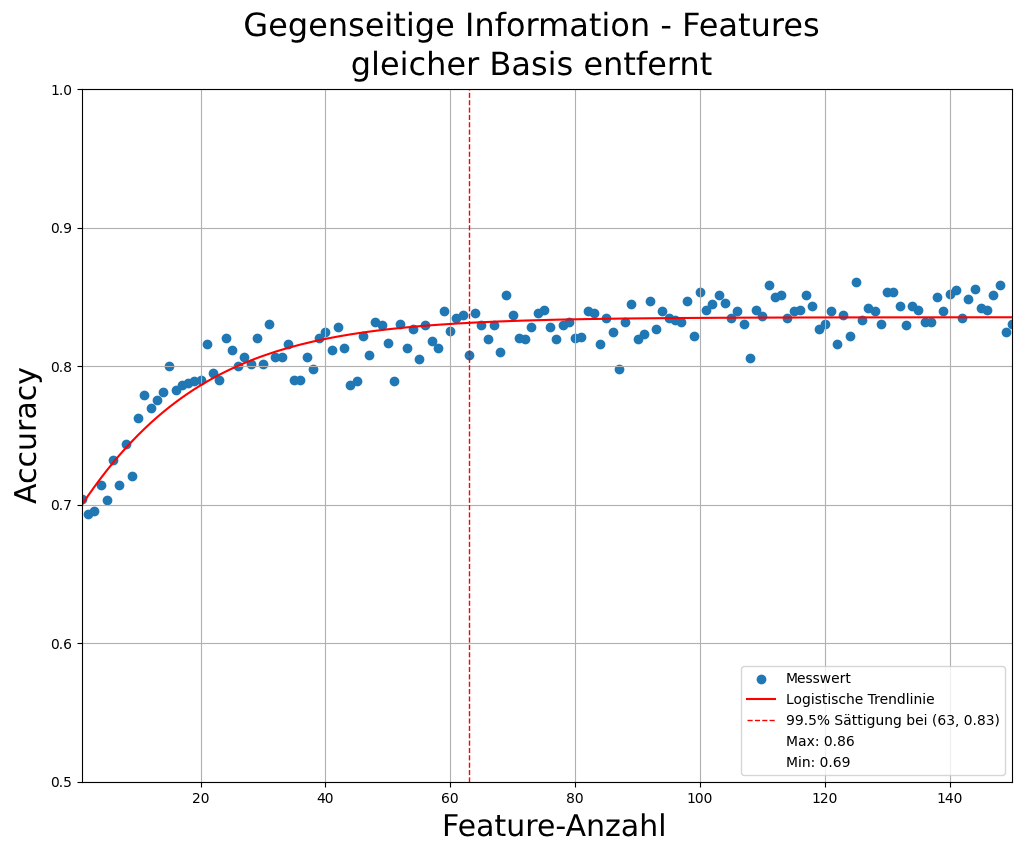
\includegraphics[width=\textwidth, height=11cm]{img/Plots/Feature Auswahl/Filter-Methoden Mutual Info mit Entfernen.png}
         \caption{Gegenseitige Infomation}
     \end{subfigure}
     \caption{Verlauf der Accuracy nach dem Entfernen von Features mit gleicher Basis.}
     \label{fig:plotRIPsame Bais}
\end{figure}

\begin{figure}[hp]
     \centering
     \begin{subfigure}[b]{0.9\textwidth}
         \centering
         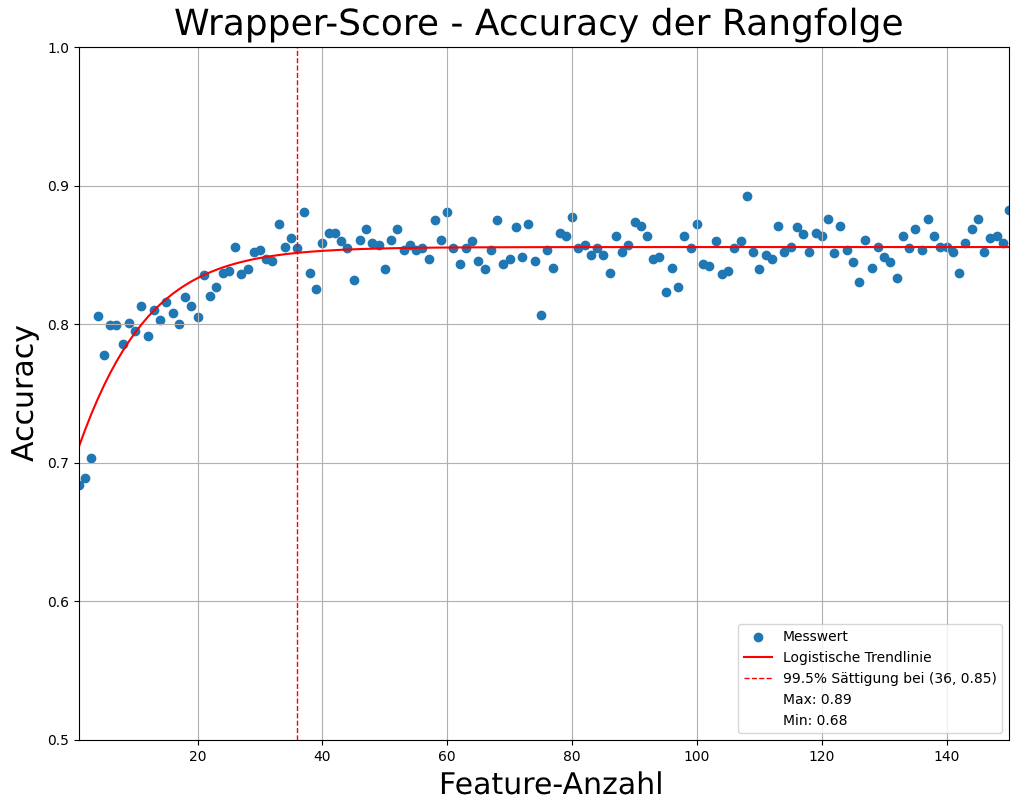
\includegraphics[width=\textwidth, height=11cm]{img/Plots/Feature Auswahl/Wrapper-Score.png}
         \caption{Wrapper-Score voher}
     \end{subfigure}
     \hfill
     \begin{subfigure}[b]{0.9\textwidth}
         \centering
         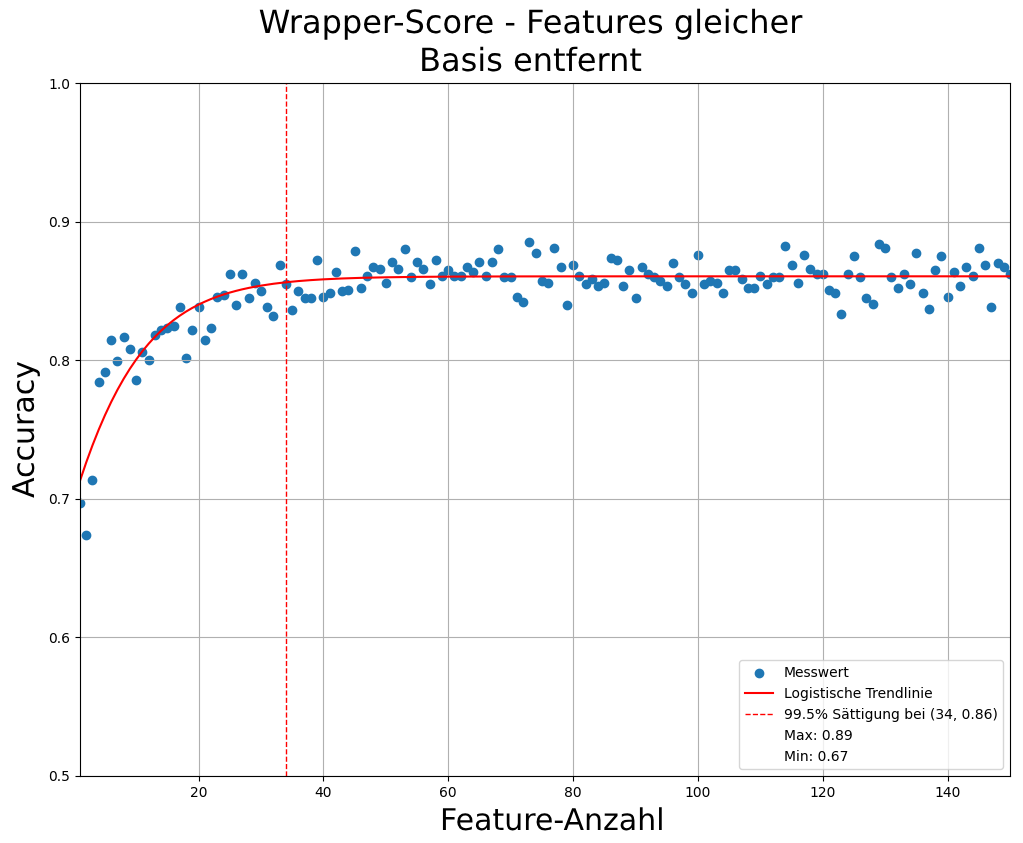
\includegraphics[width=\textwidth, height=11cm]{img/Plots/Feature Auswahl/Wrapper-Score mit Entfernen.png}
         \caption{Wrapper-Score nachher}
     \end{subfigure}
     \caption{Verlauf der Accuracy nach dem Entfernen von Features mit gleicher Basis.}
     \label{fig:plotRIPsame Bais Wrap}
\end{figure}

Die Rangfolgen werden überarbeitet, wobei nur das am höchsten bewertete Feature, das auf dem gleichen Basis-Feature aufbaut in der Rangfolge verbleibt Dadurch soll Redundanz reduziert werden. In der Abbildung \ref{fig:plotRIPsame Bais} sind die entsprechenden Plots zu den Rangfolgen der Filter-Methoden zu sehen und in Abbildung \ref{fig:plotRIPsame Bais Wrap} sind die des Wrapper-Scores zu sehen. In Tabelle \ref{tab:entfSameBasis} befindet sich ein tabellarischer Vergleich.

\begin{table}[htbp]
\centering
\caption{Vergleich der Sättigungspunkte nach entfernen von Features gleicher Basis.}
\label{tab:entfSameBasis}
\begin{tabular}{
  >{\raggedright\arraybackslash}p{0.4\linewidth}
  S[table-format=2.0]
  S[table-format=3.0]
}
\toprule
{Methode} & {Accuracy [\%]} & {Featureanzahl} \\
\midrule
Varianzanalyse & 83 & 44 \\
gegenseitige Information & 83 & 63 \\
Wrapper-Score & 86 & 34 \\
\bottomrule
\end{tabular}
\end{table}

Es ist zu sehen, dass sich das Entfernen von Features mit gleicher Basis auf alle Feature-Rangfolgen positiv ausgewirkt. Es wird eine bessere Accuracy mit weniger Features erreicht. Somit lässt sich sagen, dass tatsächlich Redundanzen entfernt werden, wodurch eine Feature-Menge entsteht, welche dem Modell mehr Information bietet als zuvor.

\clearpage
\subsection{Performancevergleich der Feature-Kategorien}
Aus der Rangfolge des Wrapper-Scores werden nur bestimmte Feature-Kategorien und Kombinationen von Kategorien getestet. Die Verläufe der Accuracy sind in Abbildung \ref{fig:plotCompKateg} zu sehen. Eine tabellarische Darstellung befindet sich in Tabelle \ref{tab:comKate}.

\begin{figure}[htb]
     \centering
     \begin{subfigure}[b]{\textwidth}
         \begin{subfigure}[b]{0.49\textwidth}
             \centering
             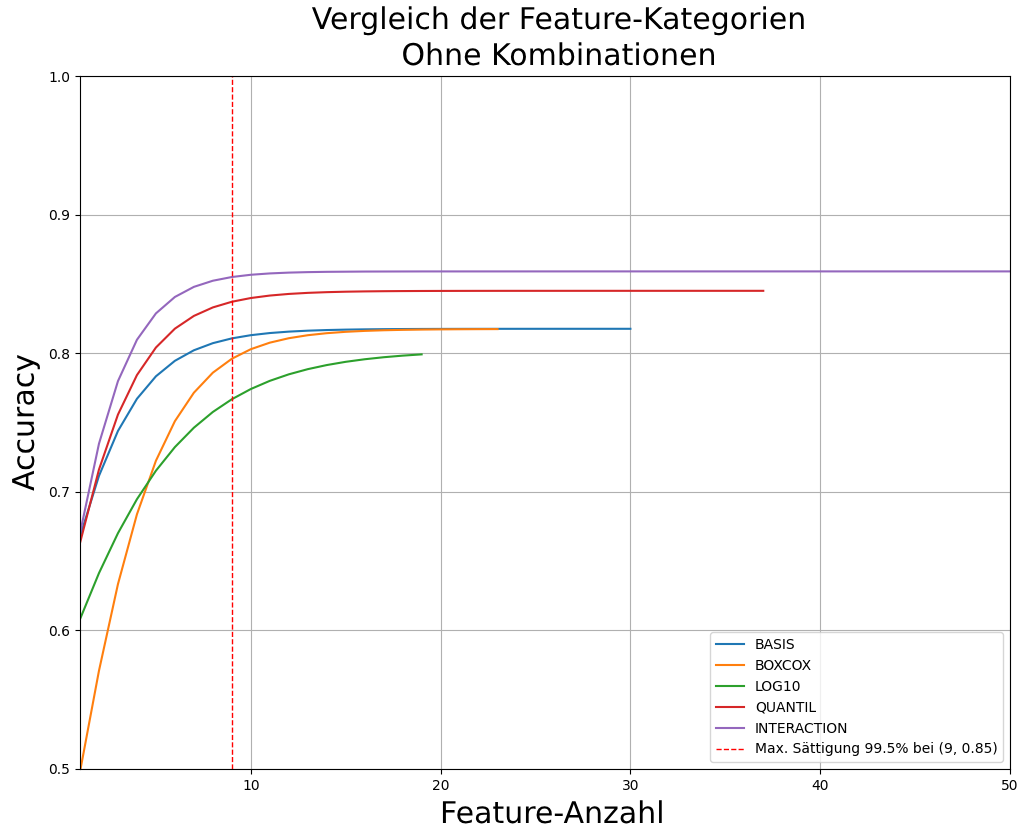
\includegraphics[width=\textwidth]{img/Plots/Feature Auswahl/Trendlinien Feature-Kategorien 0Up- Accuracy Plot.png}
             \caption{Keine Kombinationen}
         \end{subfigure}
         \hfill
         \begin{subfigure}[b]{0.49\textwidth}
             \centering
             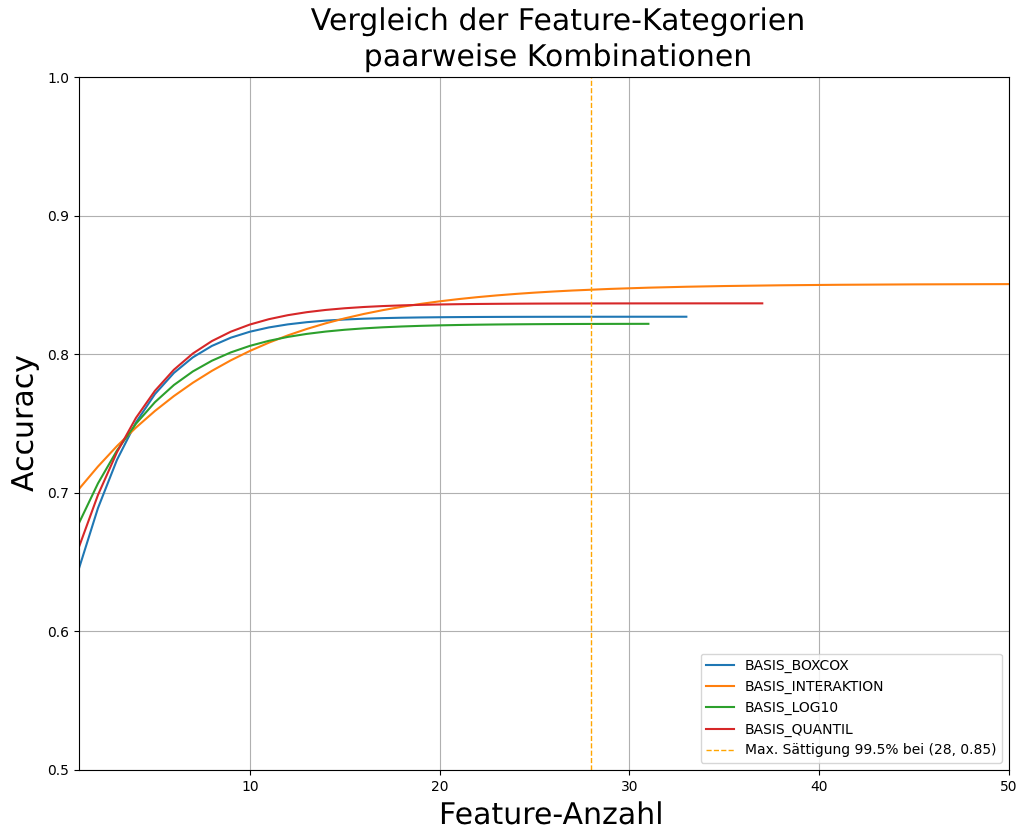
\includegraphics[width=\textwidth]{img/Plots/Feature Auswahl/Trendlinien Feature-Kategorien 1Up - Accuracy Plot.png}
             \caption{Einfache Kombinationen}
         \end{subfigure}
     \end{subfigure}
     \hfill
     \begin{subfigure}[b]{\textwidth}
         \begin{subfigure}[b]{0.49\textwidth}
             \centering
             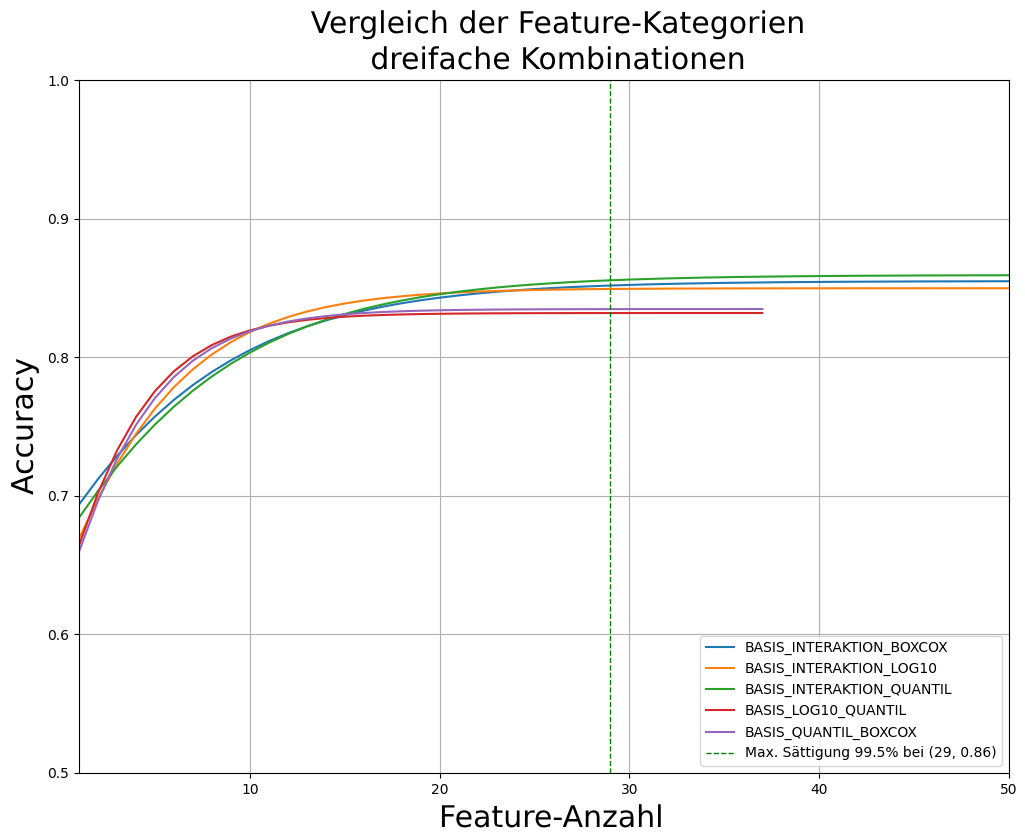
\includegraphics[width=\textwidth]{img/Plots/Feature Auswahl/Trendlinien Feature-Kategorien 2Up - Accuracy Plot.png}
             \caption{Zweifache Kombinationen}
         \end{subfigure}
         \hfill
         \begin{subfigure}[b]{0.49\textwidth}
             \centering
             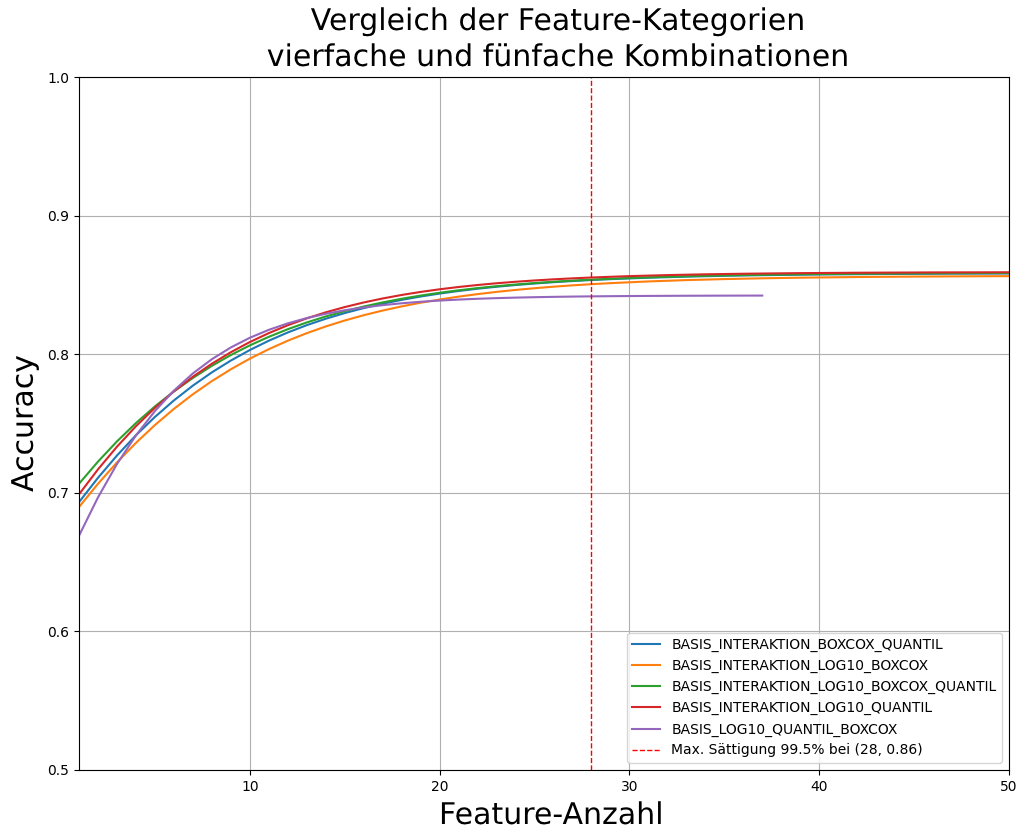
\includegraphics[width=\textwidth]{img/Plots/Feature Auswahl/Trendlinien Feature-Kategorien 3Up - Accuracy Plot.png}
             \caption{Vier- und fünffache Kombinationen}
         \end{subfigure}
     \end{subfigure}
     \caption{Verlauf der Accuracy von unterschiedlichen Kombinationen der Feature-Kategorien.}
     \label{fig:plotCompKateg}
\end{figure}

\begin{table}[htbp]
\centering
\caption{Vergleich der Sättigungspunkte unterschiedlicher Kategorie-Kombinationen}
\label{tab:comKate}
\begin{tabular}{
  >{\raggedright\arraybackslash}p{0.5\linewidth}
  S[table-format=2.0]
  S[table-format=2.0]
}
\toprule
{Kombination} & {Accuracy [\%]} & {Featureanzahl} \\
\midrule
Basis & 81 & 11 \\
Interaktion & 85 & 9 \\
Quantil & 84 & 11 \\
Log & 82 & 16 \\
BoxCox & 81 & 14 \\
\midrule
Basis-Interaktion & 85 & 28 \\
Basis-Quantil & 83 & 15 \\
Basis-Log & 82 & 16 \\
Basis-BoxCox & 82 & 13 \\
\midrule
Basis-Interaktion-Quantil & 86 & 29 \\
Basis-Interaktion-Log & 85 & 20 \\
Basis-Interaktion-BoxCox & 85 & 28 \\
Basis-Quantil-Log & 83 & 14 \\
Basis-Quantil-BoxCox & 83 & 15 \\
Basis-Log-BoxCox & 82 & 14 \\
\midrule
Basis-Interaktion-Quantil-Log & 86 & 28 \\
Basis-Interaktion-Quantil-BoxCox & 85 & 30 \\
Basis-Interaktion-Log-BoxCox & 85 & 31 \\
Basis-Quantil-Log-BoxCox & 84 & 20 \\
\midrule
Basis-Interaktion-Quantil-Log-BoxCox & 85 & 30 \\
\bottomrule
\end{tabular}
\end{table}

Es ist zu sehen, dass die höchste Accuracy mit der Kombination aus den Basis-Features, den Interaktionsfeatures und den Quantil-Features erreicht wird. Das Hinzufügen logarithmischen Features verschlechtert die Wertung nicht, jedoch zeigt dies auch, dass auf die logarithmischen Features verzichtet werden kann. Auf die Box-Cox-Features werden für das Modul nicht verwendet.\par


\subsection{Untersuchungen zur Modellauswahl} \label{sec:ErgebModSelEval}
Die Abbildung \ref{fig:plotCompModel} zeigt die Plots der Accuracy zu den unterschiedlichen Modellen. In Tabelle \ref{tab:compModel} ist der Vergleich der Sättigungspunkte zu sehen.

\begin{figure}[p]
     \centering
     \begin{subfigure}[b]{0.9\textwidth}
         \begin{subfigure}[b]{0.49\textwidth}
             \centering
             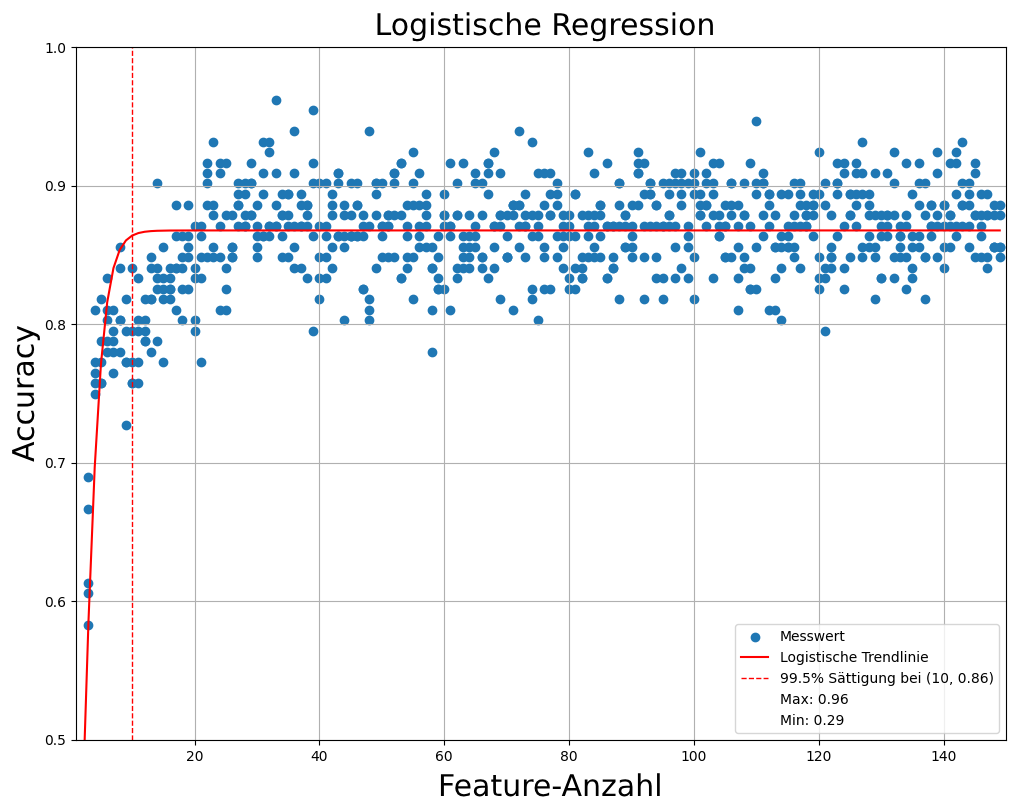
\includegraphics[width=\textwidth, height=5cm]{img/Plots/Modell Auswahl/Logistic Regression - Accuracy Plot.png}
             \caption{Logistische Regression}
         \end{subfigure}
         \hfill
         \begin{subfigure}[b]{0.49\textwidth}
             \centering
             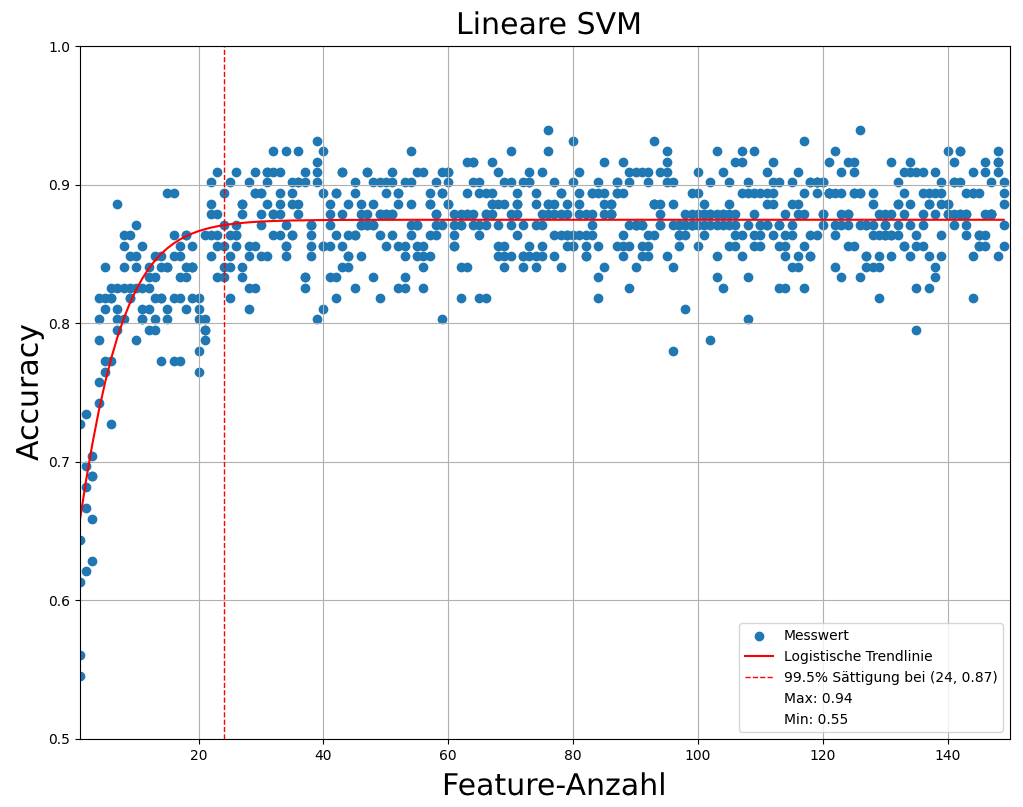
\includegraphics[width=\textwidth, height=5cm]{img/Plots/Modell Auswahl/Linea SVM - Accuracy Plot.png}
             \caption{Lineare SVM}
         \end{subfigure}
     \end{subfigure}
     \hfill
     \begin{subfigure}[b]{0.9\textwidth}
         \begin{subfigure}[b]{0.49\textwidth}
             \centering
             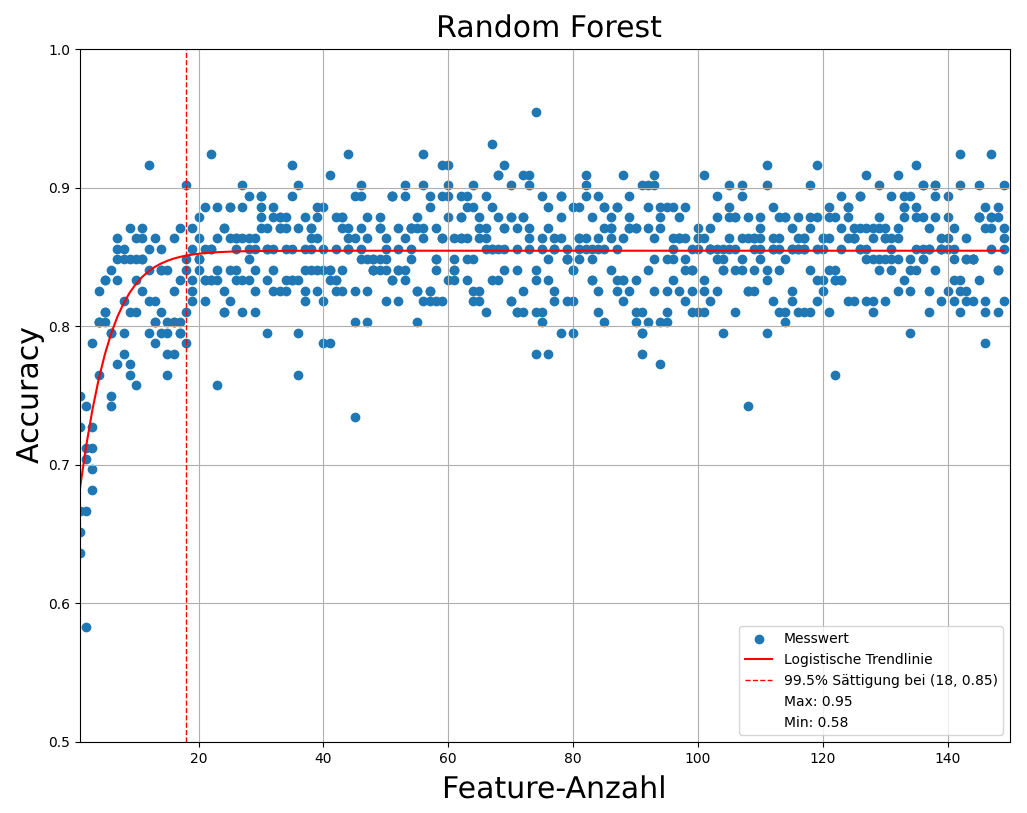
\includegraphics[width=\textwidth, height=5cm]{img/Plots/Modell Auswahl/Random Forest - Accuracy Plot.png}
             \caption{Random Forest}
         \end{subfigure}
         \hfill
         \begin{subfigure}[b]{0.49\textwidth}
             \centering
             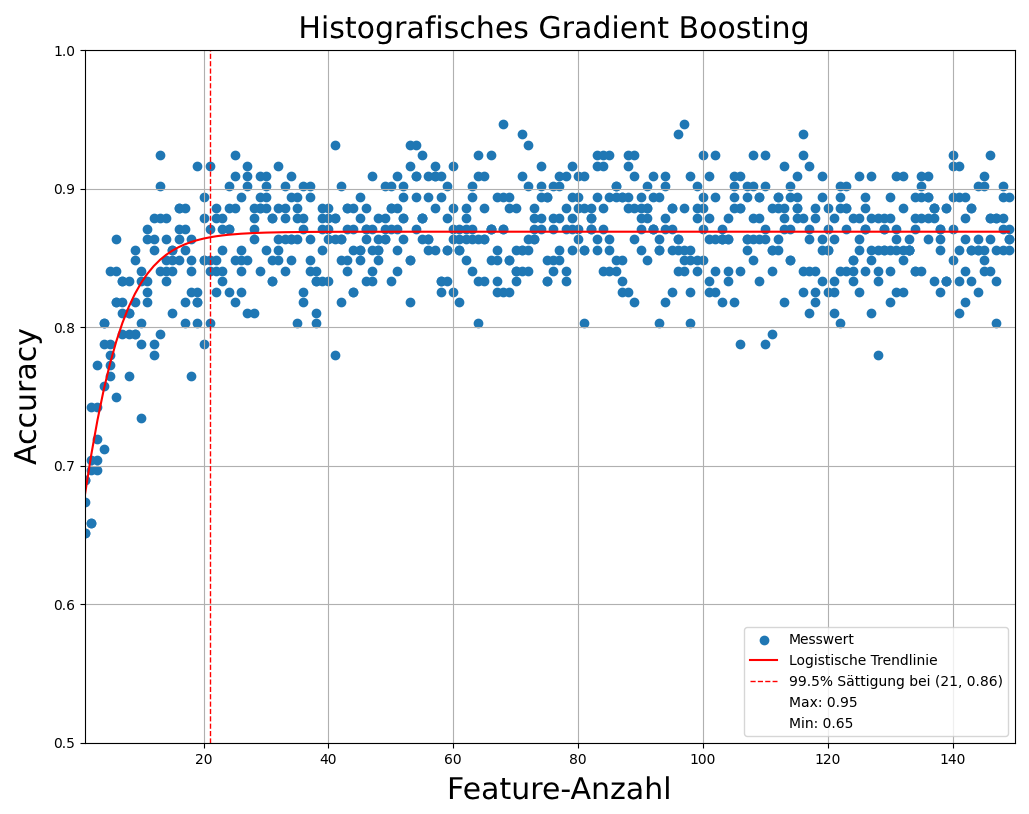
\includegraphics[width=\textwidth, height=5cm]{img/Plots/Modell Auswahl/Hist Gradien Boosting - Accuracy Plot.png}
             \caption{Histografisches Gradient Boosting}
         \end{subfigure}
     \end{subfigure}
     \begin{subfigure}[b]{0.9\textwidth}
         \centering
         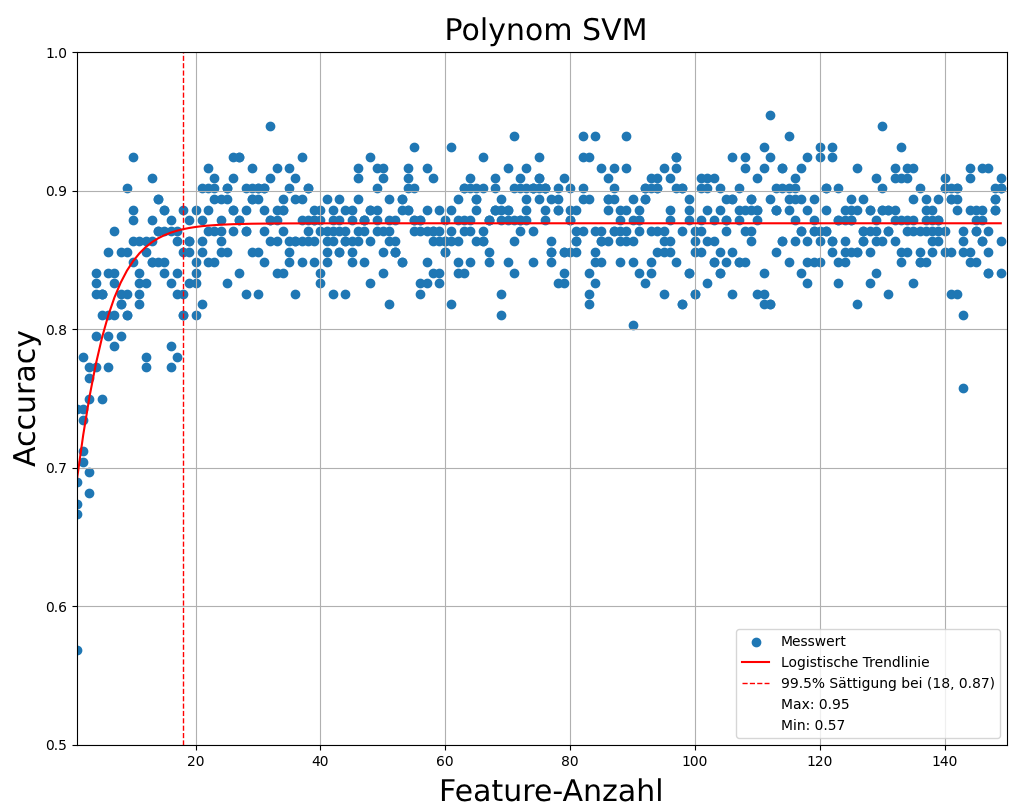
\includegraphics[width=\textwidth, height=10cm]{img/Plots/Modell Auswahl/poly SVM - Accuracy Plot.png}
         \caption{Polynomiale SVM}
     \end{subfigure}
     \caption{Verlauf der Accuracy der unterschiedlichen Modelle.}
     \label{fig:plotCompModel}
\end{figure}

\begin{table}[htbp]
\centering
\caption{Vergleich der verschiedenen Modelle}
\label{tab:compModel}
\begin{tabular}{
  >{\raggedright\arraybackslash}p{0.5\linewidth}
  S[table-format=2.0]
  S[table-format=2.0]
}
\toprule
{Modelle} & {Accuracy [\%]} & {Featureanzahl} \\
\midrule
logistische Regression & 86 & 10 \\
lineare SVM & 87 & 24 \\
polynomiale SVM & 87 & 18 \\
Random Forest & 85 & 18 \\
Histografisches Gradient Boosting & 86 & 21 \\
\bottomrule
\end{tabular}
\end{table}

Es ist zu sehen, dass nach der Hyperparameter-Suche kaum Unterschiede in der Performance der Modelle vorhanden ist. Die niedrigste Feature-Anzahl benötigt die logistische Regression. Bei  der Betrachtung von Abbildung \ref{fig:plotCompModel} wirkt es jedoch so, dass die Sättigungskurve hier den Verlauf nicht richtig approximiert. Der tatsächliche Sättigungspunkt wird ebenfalls bei ca. 20 Features erreicht. Am besten schneiden die SVMs ab. Die polynomiale SVM erreicht die Sättigung mit einer etwas kleineren Feature-Anzahl als die lineare SVM. Aus diesem Grund fällt die Entscheidung auf die polynomiale SVM.

Die Abbildung \ref{fig:plotTrainTestFinal} zeigt den Vergleich der Accuracy des Trainings, der Validierung und des Testens. Es ist zu sehen, dass die Werte eng beieinander  verlaufen. Dadurch ist auszuschließen, dass das Modell overfittet. Es ist üblich und zu erwarten, dass der Trainingswert etwas besser ist als der Validierungswert und der Testwert. 

\begin{figure}[htb]
    \centering
    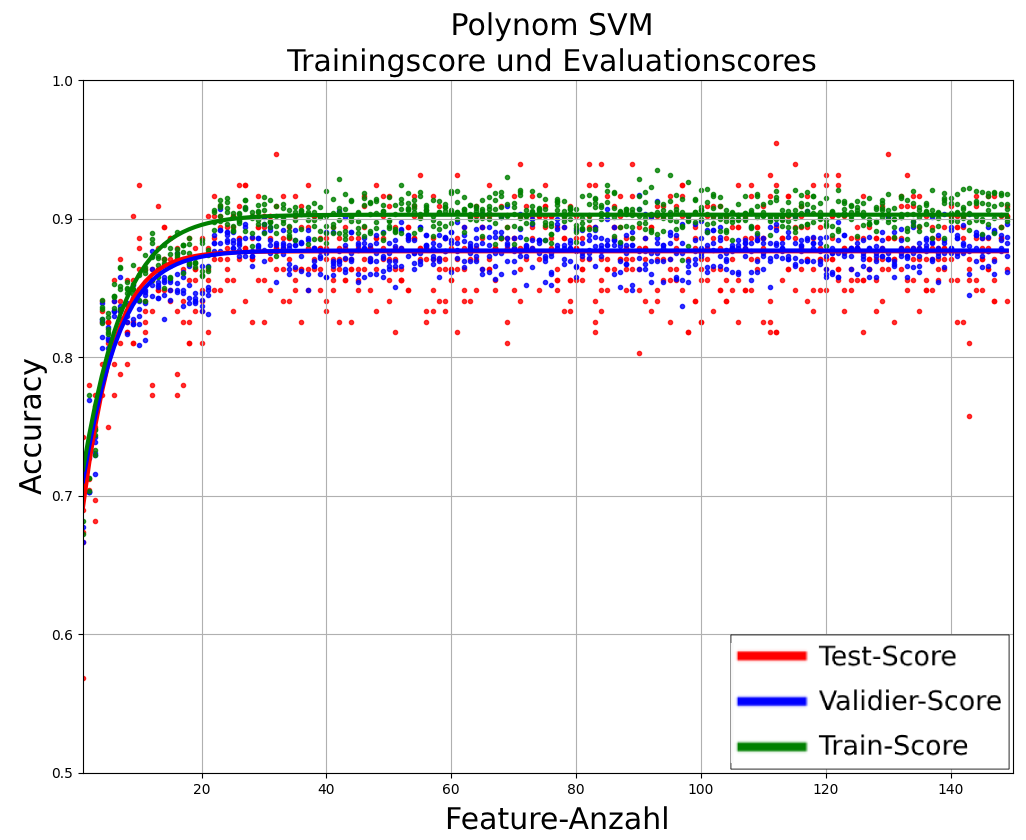
\includegraphics[width=0.9\textwidth]{img/Plots/Modell Auswahl/poly SVM - Comparation Plot.png}
    \caption{Verlauf der Accuracy des Trainings, der Validierung und des Testens des finalen Modells.}
    \label{fig:plotTrainTestFinal}
\end{figure}

Die Tabelle \ref{tab:KonfMatr} zeigt die Konfusionsmatrix des finalen Tests.

\begin{table}[htbp]
    \centering
    \caption{Konfusionsmatrix des Testens des finalen Modells.}
    \label{tab:KonfMatr}
    \begin{tabular}{l|rrr|r}
        \toprule
        \multirow{1}{*}{\textbf{Echtes Verhalten}} & \multicolumn{3}{c|}{\textbf{Geschätztes Verhalten}} & {\textbf{Gesamt}}\\
        %\cmidrule(lr){2-4}
         & Kampf & Kontrollgang & Normalverhalten & \\
        \midrule
        Kampf                & 82,0\, \% &  2,6\, \% & 16,0\, \% & 100 \%\\
        Kontrollgang         &  2,3\, \% & 98,0\, \% &  0,0\, \% & 100 \%\\
        Normalverhalten      & 12,0\, \% &  0,0\, \% & 88,0\, \% & 100 \%\\
        \bottomrule
    \end{tabular}
\end{table}

\clearpage
\subsection{Fazit der Untersuchungen zur Feature-Auswahl und der Modellauswahl}
Die Verwendung des Wrapper-Scores zur Ermittlung der Feature-Rangfolge hat sich als überlegen gegenüber den Filter-Methoden erwiesen. Dies bestätigt, dass der Wrapper-Score multivariate Einflüsse unabhängig vom Modell berücksichtigt. Das Entfernen von Features, die sich die Basis teilen, reduziert Redundanz und verbessert die Feature-Rangfolge. Für eine gute Performance ist es ausreichend nur die Basis-Features, die Quantil-Features und die Interaktionsfeatures zu ermitteln. Mit dieser Rangfolge und den eingestellten Hyperparametern sind nur kleine Unterschiede in der Performance der Modelle festzustellen. Mit der polynomialen SVM lässt sich laut den Daten die beste Accuracy mit der kleinsten Feature-Anzahl erreichen. Dieses Modell wird ausgewählt. Um stabiler in der Sättigung zu liegen, wird die Feature-Anzahl auf 40 vergrößert.